%!TEX root = ../main.tex
\section{Streamlake Data Processing} 
\label{sec:dataeva}

In this Section, we present the data processing services  in the data layer. Driven by practical application scenarios discussed in Section~\ref{sec:motivation}, these services provide a comprehensive, enterprise-level data lake storage solution  to efficiently store and process  log messages at scale. The StreamLake services encompass a stream storage system for message streaming (Section~\ref{subsec:stream}), lakehouse-format read/write capabilities for efficient tabular data processing (Section~\ref{subsec:lakehouse}), and support for query operator computation pushdown(Section~\ref{subsec:pushdown}).


\subsection{Message Streaming}~\label{subsec:stream}
We develop a  distributed stream storage engine that facilitates message streaming at large scale. Our engine leverages the stream object storage abstraction to ensure enterprise-level reliability and scalability.


\noindent\textbf{Overall architecture of streaming service.} The high-level design of the stream service is shown in Figure~\ref{fig:service}. The stream storage system comprises of producers, consumers, stream workers, stream objects, and a stream dispatcher, which work together to provide seamless message streaming.

\cc{which techniques to ensure reliability and scalability? Here, can we summarize something different (our characteristic) ?}


\begin{figure}[htbp]
	
	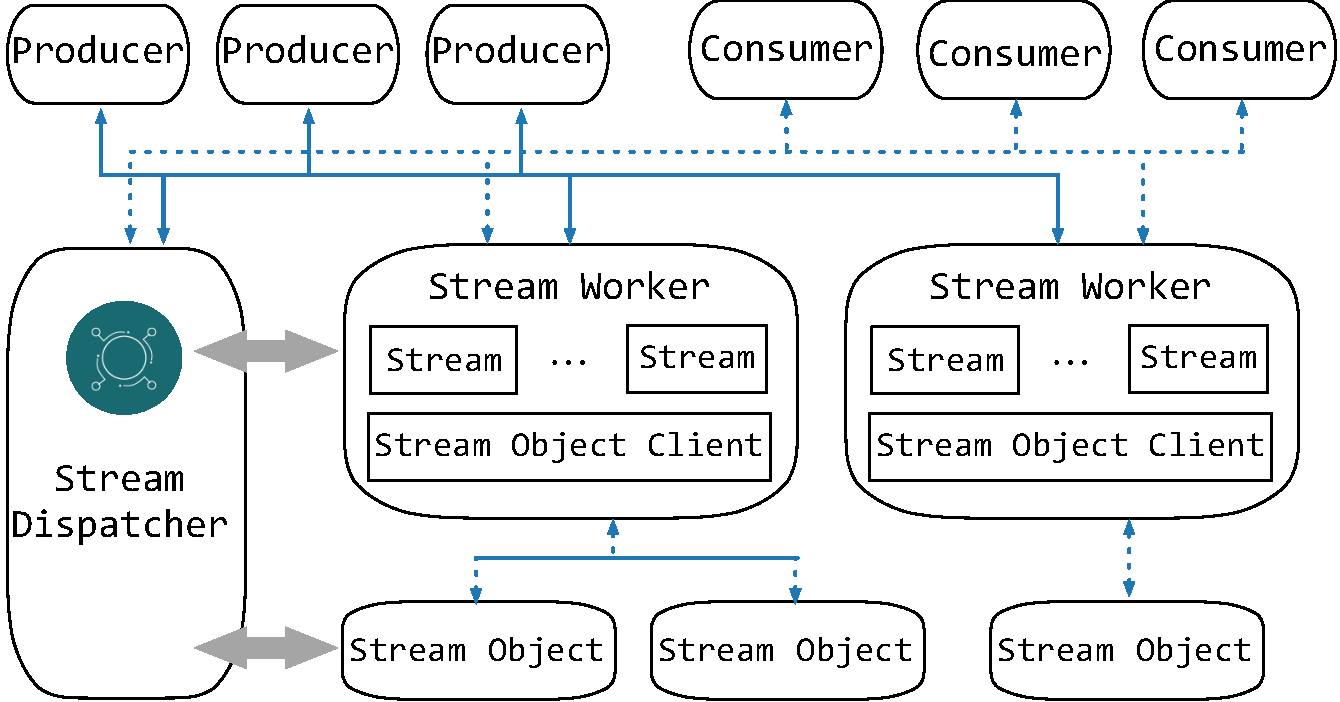
\includegraphics[scale=0.4]{figures/streamservice}
	\centering
	\vspace{-1em}
	\caption{Write Message to \sys.}
	\label{fig:service}
	\vspace{-1em}
\end{figure}

\noindent\underline{\textit{Producers and Consumers.}} Producers are responsible for publishing messages to topics, which are named resources for categorizing streaming messages. Consumers, located downstream, subscribe to these topics to receive and process the published messages. To ensure seamless integration with existing open-source message streaming services used by our customers in production environments, the producer and consumer message APIs are designed to be compatible with the open-source de facto standard. This maximizes connectivity with the ecosystem, allowing users to easily migrate their applications to \sys with minimum costs. Figure~\ref{fig:producer}  demonstrates the process of writing and reading messages using the producer and consumer APIs. In this example, a producer writes a new message ``Hello World'' as a key-value pair to a topic named ``\texttt{topic\_streamlake\_tes}''. The consumer then subscribes to this topic and processes published messages.

\begin{figure}[htbp]
	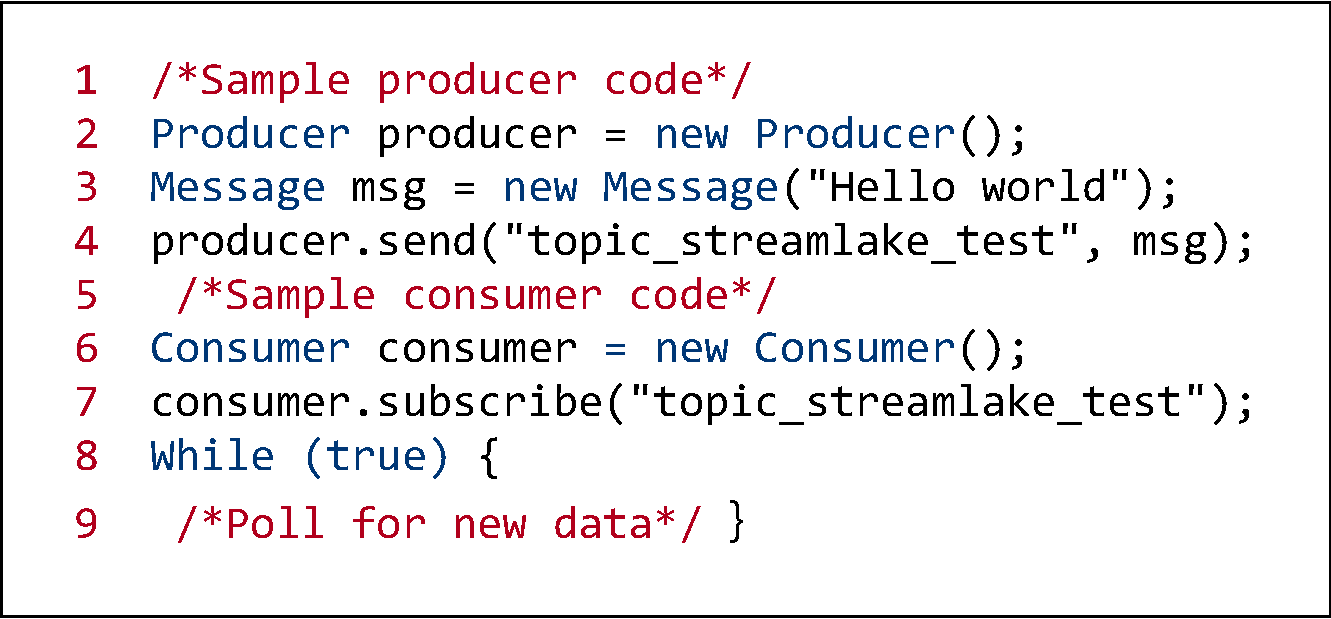
\includegraphics[scale=0.3]{figures/producer}
	\centering
	\vspace{-1em}
	\caption{Sample code of Producer and Consumer.}
	\label{fig:producer}
	\vspace{-1em}
\end{figure}

\noindent\underline{\textit{Stream workers}} work together with stream objects discussed in Section~\ref{subsec:streamobject} to tackle stream processing and message storage. The number of stream workers is determined by configurations and the physical resources allocated to the stream storage. Each stream worker is capable of handling multiple streams\footnote{streams? Above we talk about messages} and a single stream object client. When a topic is created, streams are added to the stream workers in a round-robin manner to ensure even distribution and workload balancing across the cluster.

Each stream is mapped to a unique stream object in the storage layer, which is a  storage abstraction customized to  key-value message streaming. The stream object offers efficient interfaces and implementations for writing and reading streams from the storage pools. The persistence process is detailed in Figure~\ref{fig:write}.

The task of message delivery is carried out by stream object clients, which monitor the stream objects. These clients unwrap messages from clients, encapsulate them in the stream object data format, and redirect them to the corresponding stream objects via RDMA. To guarantee message delivery, the clients actively monitor the health of the stream objects to which they are connected and regularly exchange critical service data with the dispatcher service. This synchronization process includes reporting the health of the stream object connections and refreshing the stream objects connected to by the client.


\noindent\underline{\textit{Stream dispatcher.}} The stream dispatcher is responsible for managing the metadata and configurations of the messaging service, and directing external and internal requests to the appropriate resources for message  dispatch. The relationships among topics, streams, stream workers, and stream objects are stored as key-value pairs in a fault-tolerant key-value store within the stream dispatcher. When there is  a status change   (\eg a stream worker or topic is added or removed), the metadata  in the key-value store is updated immediately to refresh the topology tracking. This topology tracking aids the stream dispatcher in directing requests for message stream dispatch. When there is a producer or consumer connection request, the stream dispatcher will route the request to the appropriate stream worker based on the associated stream topic, establishing a direct message exchange channel between the producer, the stream worker, and the consumer.

\begin{figure}[htbp]
	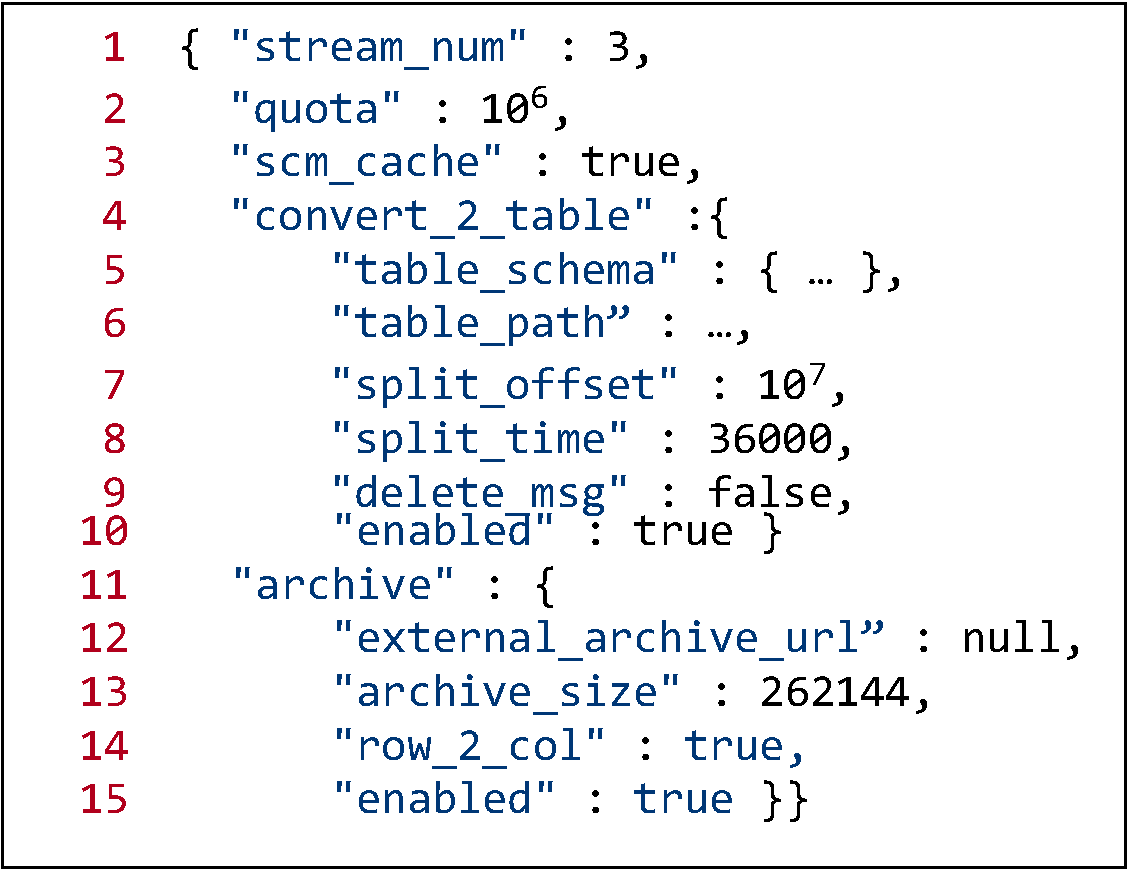
\includegraphics[scale=0.35]{figures/config}
	\centering
	\vspace{-1em}
	\caption{Stream Storage Configuration Example..}
	\label{fig:config}
	\vspace{-1em}
\end{figure}


The stream dispatcher also sets configurations for the messaging service in the unit of topic\footnote{@ what is the connection with the above? I want to ask the relationship among topic, stream, messages}. An example of  configurations is shown in Figure~\ref{fig:config}.



$\bullet$~\textit{The \texttt{stream\_num} configuration} sets the parallelism of a topic, which should be provided during topic declaration. In the example, three streams are created for the topic and they are evenly distributed among stream workers to process messages in parallel.

$\bullet$~\textit{The \texttt{quota} configuration} sets the maximum processing rate for each stream. In the example, each stream can process up to $10^6$ messages per second.

$\bullet$~\textit{The \texttt{scm\_cache} configuration} enables the use of SCM\footnote{no full name} caches.

$\bullet$~\textit{The \texttt{convert\_2\_table} configuration} enables the automatic conversion of stream object messages to table object records. When it is set, a background process will apply the \texttt{table\_schema} to convert messages to table object records periodically and save them in \texttt{table\_path}, \ie the table object directory. The conversion is triggered by either an accumulation of $10^7$ messages or the passing of 36000 seconds.

$\bullet$~\textit{The \texttt{archive} configuration} automates the archiving of historical data to meet business and regulatory requirements. Data can be stored in the cost-effective \sys archive storage pool or exported to an external storage system specified in the \textit{\texttt{external\_archive\_url} configuration}. The \textit{\texttt{archive\_size} configuration} denotes the data volume in MB that triggers archiving, and the \textit{\texttt{row\_2\_col} configuration} determines whether the data is archived in a columnar format.

\cc{The StreamLake stream storage provides guaranteed delivery, efficient transfer, and high elasticity for enterprise use.\footnote{We should build connection with the above designs.}}

\noindent\textbf{Delivery Guarantee:} Our system ensures consistent message delivery through several measures. (1) Data within a stream object is strictly ordered, ensuring that messages are consumed in the order in which they are received. (2) Message writing is idempotent, which means that for network failure, duplicate messages sent by the producer  can be identified.
 (3) Strong data consistency is achieved by eliminating unreliable components like file systems and page caches, and storing data in  stream objects that can tolerant node, network, and disk failures. (4) The system provides exactly-once\footnote{@} semantics through the use of a transaction manager and the two-phase commit protocol. This tracks participant actions and ensures that all results in a transaction are visible or invisible at the same time.
 
 %There are two typical scenarios. The first is that a producer writes a batch of messages to multiple streams. All messages are either successfully written or failed. The second scenario is that the application reads the message, processes the message, and writes the message to a new stream and the whole process are either successful or failed.

\noindent\textbf{Efficient Transfer:} Our system implements several mechanisms to efficiently transfer data. First, Stream workers and stream objects are connected through a data bus\footnote{*reviewer suggest to extend} with RDMA, which reduces the switch overhead in the TCP/IP protocol stack. Second, an I/O aggregation mechanism is used to aggregate small I/O requests and increase throughput. This function can be disabled for latency-sensitive\footnote{low latency?} scenarios. Finally, a local cache is implemented at the stream object client to speed up message consumption.

\noindent\textbf{High Elasticity:} Our system provides high elasticity by decoupling data storage and data serving. The number of stream workers can be adjusted without data migration, and the mapping between stream workers and stream objects can be updated to reflect the changes in a matter of seconds. This allows the message streaming service to easily scale up or down to accommodate changes in service demand.



\subsection{Lakehouse Read and Write}~\label{subsec:lakehouse}


\subsection{Query Operator Computation Push Down}~\label{subsec:pushdown}